\chapter{Blockchain Scalability}
The \textbf{Blockchain trilemma} states that blockchain systems can only achieve two of the following three properties: decentralization, security, and scalability. This is because the three properties are in conflict with each other, and was initially stated by Vitalik Buterin.

\begin{figure}[htbp]
   \centering
   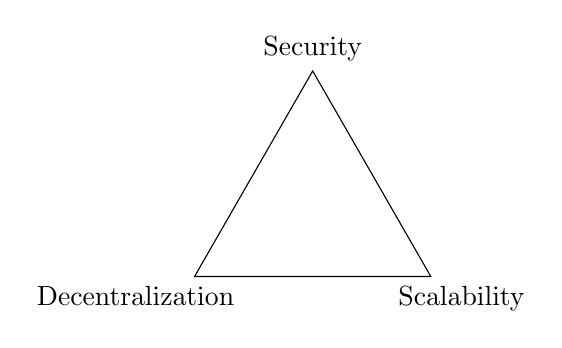
\begin{tikzpicture}[scale=3]
      \draw (0,0) -- (1,0) -- (0.5,0.87) -- cycle;
      \node at (1.13,0) [below] {Scalability};
      \node at (0.5,0.87) [above] {Security};
      \node at (-0.25,0) [below] {Decentralization};
      % \node at (0.5,0.4) {Blockchain Trilemma};
  \end{tikzpicture}
  \caption{Blockchain Trilemma}
   \label{fig:blockchain_trilemma}
\end{figure}

\section{``On-chain'' Scalability}
\textbf{On-chain} scalability refers to the ability of a blockchain to handle a large number of transactions per second. The Bitcoin network can handle 7 transactions per second, while the Ethereum network can handle 15 transactions per second. This is a very low number compared to traditional payment systems like Visa, that can handle 24,000 transactions per second.\\
Besides note that in Bitcoin 7 transactions per second are handled, but they not get confirmed until 6 blocks have been mined on top of them, \ul{taking about 1 hour to actually transfer Bitcoins}.
Furthermore, the transaction fee is about 55\$ to confirm 6 blocks.

On-chain scalability solutions ---each one has pros and cons--- include:
\begin{itemize}
   \item Increase block size
   \item Increase block frequency
   \item Cross-chains and side-chains 
   \item Use alternative consensus algorithms (e.g. \textit{Proof of Stake})
\end{itemize}

\section{``Off-chain'' Scalability}
The key idea for \textbf{off-chain} scalability is to move transactions off the main blockchain, and to settle them on the main blockchain only when necessary. This way, the main blockchain is not overloaded with transactions, and only used as ``arbiter'' when necessary.

Off-chain transactions are like promissory notes, where the parties involved in the transaction exchange IOUs, and settle them on the main blockchain only later on.
The security of such transactions is almost the same of the main chain, but allow for high-volume of instant, trustless, micropayments.

Potential problems are:
\begin{itemize}
   \item Possible \textbf{Centralization}
   \item \textbf{Fund Locking}
   \item \textbf{Always on requirement}
\end{itemize}

Bitcoin Lightning Network is an example of off-chain scalability solution. It is a second layer protocol that operates on top of the Bitcoin blockchain, and allows for instant, low-fee, micropayments.
Currently the Lightning Network can handle 10,000 transactions per second, and it is growing.

\section{MultiSignature Transactions}
MultiSignature transactions are a way to increase the security of a transaction, by requiring the signature of multiple parties to spend the funds. This can be used to increase the security of off-chain transactions, by requiring the signature of a third party to settle the transaction on the main chain.

They are implemented through the \texttt{CHECKMULTISIG} script, that requires the signature of multiple parties to spend the funds.

Practical MultiSignature use cases are:
\begin{itemize}
   \item 1-of-n: a transaction requires the signature of only one party to spend the funds.
   \item 2-of-2: a transaction requires the signature of both parties to spend the funds.
   \item 2-of-3: a transaction requires the signature of two parties to spend the funds.
   \note{Commonly used for \textit{escrow contracts}}
\end{itemize}

\subsection{Escrow contracts}
An \textbf{escrow\footnote{``Escrow'' means ``deposito in garanzia'' in italian} contract} is a contract where a third party holds the funds until the conditions of the contract are met. The third party is responsible for releasing the funds to the correct party, and can be used to increase the security of a transaction.

Alice wants to buy a product from Bob, but she does not trust Bob. They can use an escrow contract to secure the transaction, by involving the third ---trusted--- party Judy:
\begin{enumerate}
   \item Alice creates a 2-of-3 MultiSignature transaction, where the funds are locked in the escrow contract.
   \item Coins are held in \textit{escrow} by Alice, Bob and Judy. \ul{Any \textit{two} of them can redeem the funds and specify the receiver} of the bitcoins
\end{enumerate}
In case there are no disputes, Alice and Bob can redeem the funds together, without involving Judy. If there is a dispute, Judy can decide who ``cheated'' and who gets the funds.\\
In either case, two transactions are needed, one from Alice to the escrow, and another one to either Bob or back to Alice.
\note{Technically one among Alice and Bob may decide to give the funds to Judy, but this is not in their interest and would be pointless.}

\section{Towards Pay-to-Script-Hash}

\texttt{multi-sig} scripts are longer than standard scripts, require more public keys to be exchanged and come with higher fees.
\texttt{Pay-to-Script-Hash} (P2SH) is a way to simplify the use of complex scripts, by hashing the script and using the hash as the address. This way, the script is not revealed until the funds are spent, and the address is shorter and easier to use, removing complexity at the sender side.

\section{Hash-time locked contracts}
\textbf{Hash-time locked contracts} are a way to secure a transaction by locking the funds until a certain time has passed, or a certain condition is met. They are used in the Lightning Network to secure off-chain transactions.
\begin{itemize}
   \item \texttt{Hash Locks} hash secret and store it in a script. Unlock the funds only if the secret is provided by the intended recipient.
   \item \texttt{Hash Time Locks} hast secret and store it in a script. Unlock the funds until a certain time has passed, or if the intended recipient provides the secret.
\end{itemize}

\begin{figure}[htbp]
   \centering
   \includegraphics[width=0.49\columnwidth]{images/bitcoin_htlc1.png}
   \includegraphics[width=0.49\columnwidth]{images/bitcoin_htlc2.png}
   \caption{Atomic Swap of different cryptocurrencies between Alice and Bob}
   \label{fig:bitcoin_htlc}
\end{figure}

Bob knows only the secret's hash \texttt{19bf...}, not secret itself \texttt{XYZ}, so he cannot redeem the funds in Alice's transaction. At this point Bob creates another HTLC using as lock the same hash, and sends it to Alice. Alice can now redeem the funds in Bob's transaction, revealing the secret \texttt{XYZ} and redeeming the funds in her transaction.
Since the secret is the same and it has been revealed, Bob can now redeem the funds in Alice's transaction.

\section{Clients against Full Nodes}
\textbf{Full nodes} are nodes that store the whole blockchain and validate all the transactions. They are the most secure way to use the Bitcoin network, but they require a lot of resources and time to set up.
For the majority of nodes it would be unfeasible to store the whole blockchain which takes up about 500GB of space, as it would be also to use substantial CPU power to validate transactions from other users.

Bitcoin exploits a \textbf{Simplified Payment Verification} (SPV) mode, where the client does not store the whole blockchain, but only the block headers (x1000 smaller). This way, the client can verify the transactions without storing the whole blockchain, but it is less secure than a full node.

\begin{figure}[htbp]
   \centering
   \includegraphics{images/bitcoin_spv.png}
   \caption{SPV client and Full node interaction}
   The SPV client sends a bloom filter to the full node, that will send back only the transactions that match the filter and Merkle tree paths, along with the block headers not already downloaded by the client.
   \label{fig:bitcoin_spv}
\end{figure}

The SPV, to check that a given transaction really belongs to a block, computes the Merkle Proof of the transaction exploiting the paths sent by the full node and lastly checks if the Merkle Root is the one expected, which is stored in the block header.